
\chapter{Expériences et résultats}

\label{ch:experiments_and_results}

La table~\ref{fig:results} montre l'ensemble des résultats obtenus par validation croisée. Les résultats selon les métriques de segmentation se trouvent à gauche, et ceusx selon les métriques de recherche d'information à droite. Sont d'abord indiqué les scores des systèmes de référence, dans la section supérieure. Ensuite, dans la section intermédiaire, nous montrons les résultats des segmenteurs basés sur chaque ensemble de traits (avec $A$ correspondant aux $n$-grammes, $B$ aux traits basés sur la théorie de la structure de l'information, $C$ sur \textit{TextTiling} et $D$ aux traits stylistiques et sémantiques). Enfin, dans la séction inférieure, nous montrons les résultats des segment

\section{Prétraitements}

Pour réduire le bruit présent dnas le corpus, nous filtrons les emails indésirables en se basant sur plusieurs critères, le premier d'entre eux étant l'encodage. Les messages qui ne sont pas encodés en UTF-8 sont retirés de la sélection. Le second critère est le type MIME : nous ne conservons que les messages en texte brut uniquement, et retirons ceux contenant du HTML ou d'autres contenus spéciaux.

De plus, nous choisissons de ne considérer que les réponses aux messages initiaux (les premiers messages d'une discussion). Ce choix est justifié par la supposition que nous faisons que le module d'alignement aura plus de difficulté à reconnaître correctement des phrases qui ont été transformés à plusieurs reprise au cours de plusieurs réponses successives. En effet, ces réposnes - qui contiendraient du texte cité d'autres messages - seraient plus probablement mal étiquetées par notre système d'annotation automatique.

Le dernier critère est la longueur. Le jeu de données étant construit à partir d'une mailing list qui peut couvrir des discussions très techniques, les utilisateurs peuvent parfois envoyer des messages contenant de nombreuses lignes de code copié-collé, des logs logiciels, des sorties de commandes bash, etc. Le nombre de ces messages est marginal, mais leur longueur pouvant être tellement disproportionné qu'ils peuvent tout de même avoir un impact négatif sur les performances du segmenteur. Par conséquent, nous excluons les messages de taille supérieure à la moyenne plus la déviation standard de la taille des messages.

Après filtrage, le jeu de données ne comporte plus que 6 821 des 33 915 messages (soit 20\%).

\section{Résultats}

\subsection{Systèmes de référence (\textit{baselines})}

La première section de la table~\ref{fig:results} montre les résultats obtenus par les deux systèmes de référence. Sans surprise, \textit{TextTiling} se montre beaucoup plus performant que l'approche basée sur une segmentation régulière, et ce selon toutes les métriques sauf le rappel.

\subsection{Segmenteurs basés sur des ensembles de traits homogènes}

La seconde section de la table~\ref{fig:results} montre les résultats pour quatre différents segmenteurs, chacun entraîné avec un ensemble de traits distinct. La fonction $\phi$ est la fonction de classification, ses paramètres sont des traits, et sa sortie une prédiction. Tandis que tous les classifieurs batent sans problème le système de segmentation régulière, et rivalisent avec \textit{TextTiling} en ce qui concerne les métriques de recherche d'information, seuls le segmenteur thématique et celui basé sur les $n$-grammes parviennent à le surpasser quand la performance est mesurée par les métriques de segmentation. En termes de scores de RI, le classifieur utilisant les $n$-grammes en particulier sort du lot en ce qu'il parvient à atteindre une précision exceptionnelle de 100\%, bien que ce résultat est mitigé par un maigre rappel (39\%). Il est également intéressant de noter que le classifieur thématique, basé seulement sur la connaissance contextuelle des prédictions de \textit{TextTiling}, surpasse la sortie brute de l'algorithme.

\begin{figure}[h!]
	\centering
	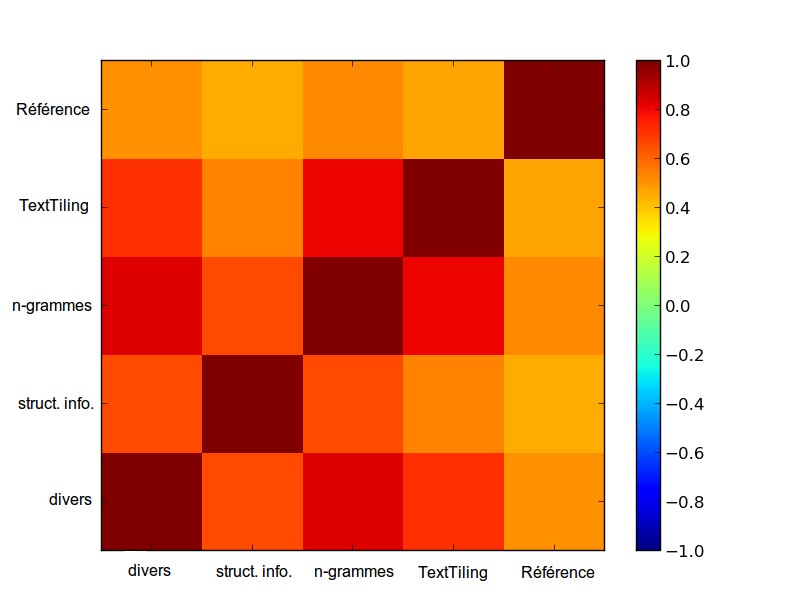
\includegraphics[width=\textwidth]{correlation.png}
	\caption{Matrice de corrélation pour les sorties des segmenteurs basés sur des ensembles de traits homogènes.}
\end{figure}

\subsection{Segmenteurs basés sur des combinaisons d'ensembles de traits}

La dernière section de la table~\ref{fig:results} montre les résultats pour quatre différents segmenteurs. 

Le premier, $\phi(A + B + C + D)$, est un simple classifieur qui prend en compte tous les traits disponibles. Ses résultats sont exactement identiques à ceux du classifieur $n$-grammes, ce qui est probablement dû au fait que les autres traits sont noyés dans la masse de traits lexicaux (1000 $n$-grammes sont pris en compte). 

Le second, $\phi(\phi(A) + \phi(B) + \phi(C) + \phi(D))$, utilise comme traits les sorties des quatre classifieurs entraînés sur des ensembles de traits différents décrits dans la sous-section précédente. Les résultats montrent que cette approche n'est pas significativement plus intéressante. 

Le troisième, $\phi(A) \cup \phi(B + C + D)$, segmente selon l'union des frontières détectées par un classifieur entraîné sur les $n$-grammes et celles identifiées par un classifieur entraîné sur tous les autres traits. Cette idée est motivée par le fait que nous savons que toutes les frontières trouvées par le classifieur basé sur les $n$-grammes sont correctes ($P=1$). Cette approche nous permet d'obtenir le meilleur rappel possible ($R=.69$), mais en contrepartie d'une bonne précision ($P=.58$). 

Le dernier, $\phi(A) \cup \delta(\phi(B + C + D))$, tente d'améliorer le rappel du classifieur basé sur les $n$-grammes sans sacrifier trop de précision en se montrant plus sélectif en acceptant de nouvelles frontières. La fonction $\delta$ est la fonction de sélection, qui ignore les frontières prédites avec une faible confiance. Seules celles identifiées par le classifieur basé sur les $n$-grammes et celles identifiées avec un taux de confiance d'au moins .99 par un classifieur entraîné sur tous les autres traits sont prises en considération. Ce système obtient des performances supérieures à tous les autres à la fois en terme de scores de segmentation et de $F_1$, cependant il reste relativement conservateur et le ratio de segmentation (le nombre de frontières prédites divisé par le nombre de frontières réelles) reste significativement plus bas que voulu, à 0.67. Jouer avec le taux de confiance minimum ($c$) permet d'ajuster $P$ de .58 ($c = 0$) à 1 ($c = 1$) et $R$ de .39 ($c = 1$) à .69 ($c = 0$).

\medskip\noindent

\begin{table}
	\begin{tabularx}{\textwidth}{c *{6}{Y}}
		\toprule
		\multicolumn{1}{l}{} 
		& \multicolumn{3}{c}{Métriques de seg.}  
		& \multicolumn{3}{c}{Métriques de RI}\\
		\multicolumn{1}{l}{} 
		& $WD$ & $P_{k}$ & $GHD$ & $P$ & $R$ & $F_1$ \\
		\midrule
		Segmentation régulière & .59 & .25 & .60 & .31 & .49 & .38  \\ 
		TextTiling & .41 & .07 & .38 & .75 & .44 & .56 \\
		\midrule
		$\phi(A)$ with $A$ = $n$-grammes & .38 & \textbf{.05} & .39 & \textbf{1} & .39 & .56 \\ 
		$\phi(B)$ with $B$ = structure info. & .43 & .11 & .38 & .60 & .68 & \textbf{.64} \\ 
		$\phi(C)$ with $C$ = TextTiling & .39 & .05 & .38 & .94 & .40 & .56 \\ 
		$\phi(D)$ with $D$ = traits divers & .41 & .09 & .38 & .69 & .49 & .57 \\
		\midrule
		$\phi(A + B + C + D)$ & .38 & \textbf{.05} & .39 & \textbf{1} & .39 & .56 \\ 
		$\phi(\phi(A) + \phi(B) + \phi(C) + \phi(D))$ & .38 & .06 & .36 & .81 & .47 & .59 \\ 
		$\phi(A) \cup \phi(B + C + D)$ & .45 & .12 & .40 & .58 & \textbf{.69} & .63 \\ 
		$\phi(A) \cup \delta(\phi(B + C + D))$ & \textbf{.36} & .06 & \textbf{.34} & .80 & .53 & \textbf{.64} \\ 
		\bottomrule
	\end{tabularx}
	\caption{Résultats comparés entre les différents systèmes de référence et les segmenteurs testés. Tous les résultats présentent \textit{WindowDiff} (\textit{WD}), $P_{k}$ et \textit{GHD} en tant que taux d'erreur, par conséquent un score bas est désirable pour ces métriques. Ceci contraste avec les trois scores de RI, pour lesquels une maigre valeur représente une faible performance. Les meilleurs scores sont indiqués en gras.}
	\label{fig:results}
\end{table}

\section{Discussion}